\documentclass[11pt]{article}

\usepackage[english]{babel}
\usepackage[utf8]{inputenc}
\usepackage{amsmath}
\usepackage{amssymb}
\usepackage{graphicx}
\usepackage[colorinlistoftodos]{todonotes}
\usepackage{listings,multicol}
\usepackage{textcomp}
\usepackage{hyperref}
\usepackage{movie15}

\setlength{\oddsidemargin}{0.5cm} \setlength{\evensidemargin}{0cm}
\setlength{\textwidth}{16cm} \setlength{\textheight}{23cm}
\setlength{\topmargin}{-0.5cm}
\textheight 21.5cm


\usepackage[numbered,framed]{matlab-prettifier}
\lstMakeShortInline"
\lstset{
  style              = Matlab-editor,
  %basicstyle         = \mlttfamily,
  escapechar         = ",
  mlshowsectionrules = true,
}


\begin{document}

\title{TEST 4 NUMERICO UCSC}

\begin{minipage}{0.15\textwidth}

\includegraphics[width=\textwidth]{ucsc.png}
\end{minipage}
\begin{minipage}{0.9\textwidth}
{UNIVERSIDAD CAT\'OLICA}\\ 
{DE LA SANT\'ISIMA CONCEPCI\'ON}\\
{DEPARTAMENTO DE MATEM\'ATICA}\\ 
{ Y F\'ISICA APLICADAS}\\
\rule{0.66\textwidth}{.5pt} Franco A. Milanese
\end{minipage}

\vspace*{0.5cm} \centerline {\bf\underline{Test 4 C\'alculo Num\'erico IN1012C }}
\centerline{\textrm{Martes 16 de junio de 2015}}  

\vspace{0.2cm}
\textbf{Nombre:} PAUTA \hspace{0.65\textwidth}\textbf{Carrera:}

\vspace{0.1cm}
\textbf{Profesor de C\'atedra:}\hspace{0.5\textwidth} \textbf{ RUT:}
 \begin{center}
 \begin{tabular}{||p{2cm}|p{2cm}|p{2cm}||}
 \hline
 Pregunta 1 &  Pregunta 2 &     Total\\
 \hline

  \vspace{1.3cm} & &       \\
 \hline
 \end{tabular}
 \end{center}

Enviar documentos solicitados en el formato solicitado al correo 
\textbf{veranonumerico@gmail.com} .
%que el ayudante le indique.
\begin{enumerate}
\item 
\begin{enumerate}
\item (20 pt.) Cree una funci\'on de Matlab llamada \texttt{2Dinterpol} que dados un conjuntos de puntos $\{(x_i,y_i)\}_{i=1}^n$ grafique el polinomio de Lagrange de las coordenadas del conjunto de puntos, pensando que son las componentes de una funci\'on
$$
\begin{array}{rcl}
\overrightarrow{x}:\mathbb{R}&\longrightarrow &\mathbb{R}^2\\
					t		& \longmapsto	& (x(t),y(t))	
\end{array},
$$
donde $\overrightarrow{x}(i)=(x_i,y_i), \quad \forall i\in\{1,\cdots,n\}$.

\item (10 pt.) En una hoja de papel semitransparente marque 15 puntos equidistantes en sentido horario del contorno de su mano izquierda, sobreponga esta hoja al monitor de su computador y usando la funci\'on \texttt{ginput()} ingrese estos puntos a Matlab. Grafique los puntos en Matlab usando asteriscos rojos. Grabe la imagen de los puntos como \texttt{puntosenmimano.jpg}.

\item (10 pt.) Use la funci\'on \texttt{2Dinterpol} para graficar la interpolaci\'on de polinomio de Lagrange de los puntos que ingres\'o a Matlab en el \'item anterior. Grabe una imagen que tenga los puntos anteriores y la curva de interpolaci\'on graficada por \texttt{2Dinterpol} como \texttt{manointerpolada.jpg}.
\end{enumerate}

Adjunte el fichero \texttt{2Dinterpol.m} y las im\'agenes \texttt{puntosenmimano.jpg}, \texttt{manointerpolada.jpg} al correo.

\textbf{Desarrollo:}
\begin{enumerate}
\item 
\begin{lstlisting}
function Dinterpol(x,y)
% Grafica la interpolacion por polinomios de Lagrange de una curva que 
% cruza por los puntos de coordenadas x,y en columnas
grado=length(x)-1;
P1=polyfit(1:length(x),x',grado)
P2=polyfit(1:length(x),y',grado);
plot(polyval(P1,1:0.1:length(x)),polyval(P2,1:0.1:length(x)));
end
\end{lstlisting}
%
\item Un c\'odigo que lee y grafica los puntos es
\begin{lstlisting}
%% Lectura de las coordenadas de los puntos de la mano
clear all; close all; clc;
[X,Y]=ginput();
%% Graficamos los puntos leidos
figure(1)
plot(X,Y,'*r');
title('Puntos en mi mano');
print('-djpeg99','puntosenmimano');
\end{lstlisting}
%
y la imagen \texttt{puntosenmimano.jpg} generada es

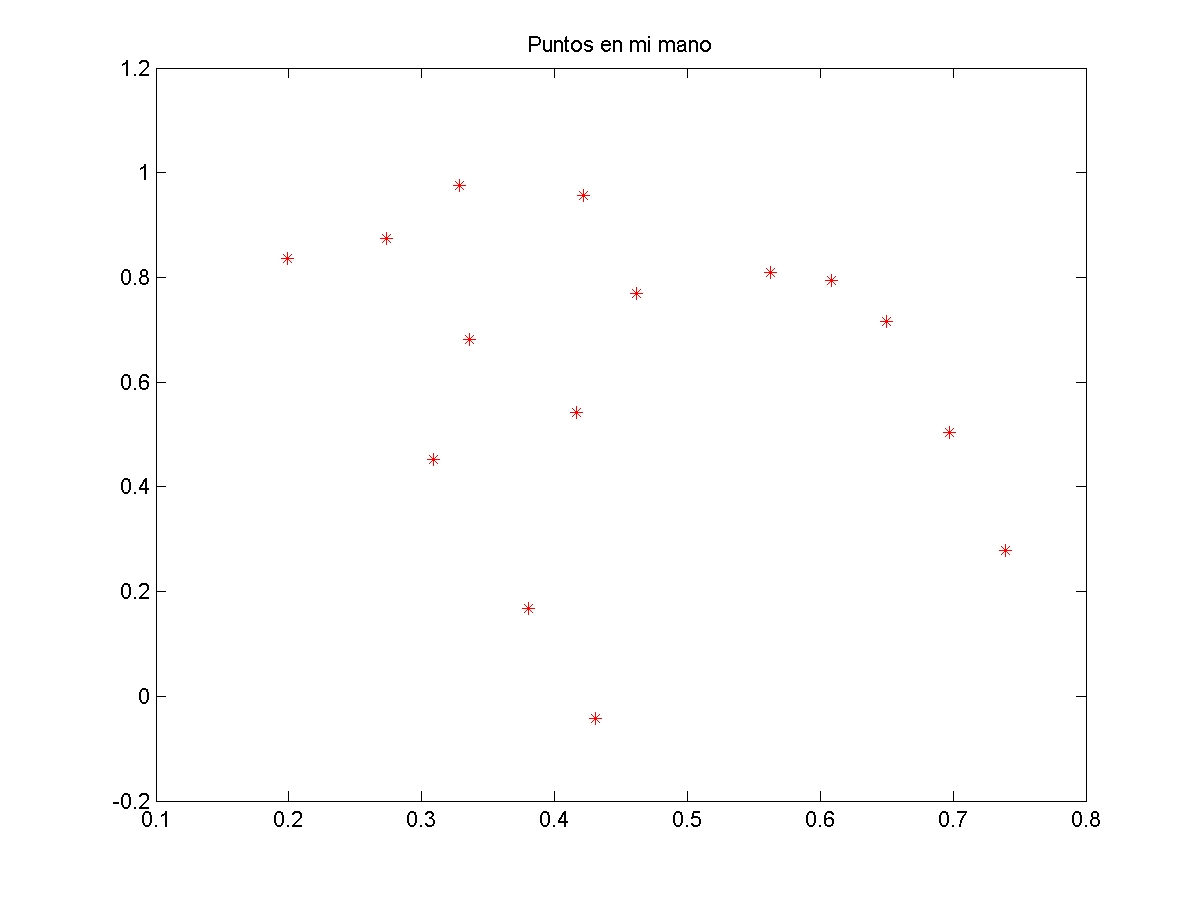
\includegraphics[width=\textwidth]{puntosenmimano.jpg}

\item 
Un c\'odigo que genera el gr\'afico pedido usando la funci\'on solicitada es
\begin{lstlisting}
figure(2)
Dinterpol(X,Y);
print('-djpeg99','manointerpolada');
\end{lstlisting}
cuya gr\'afica es

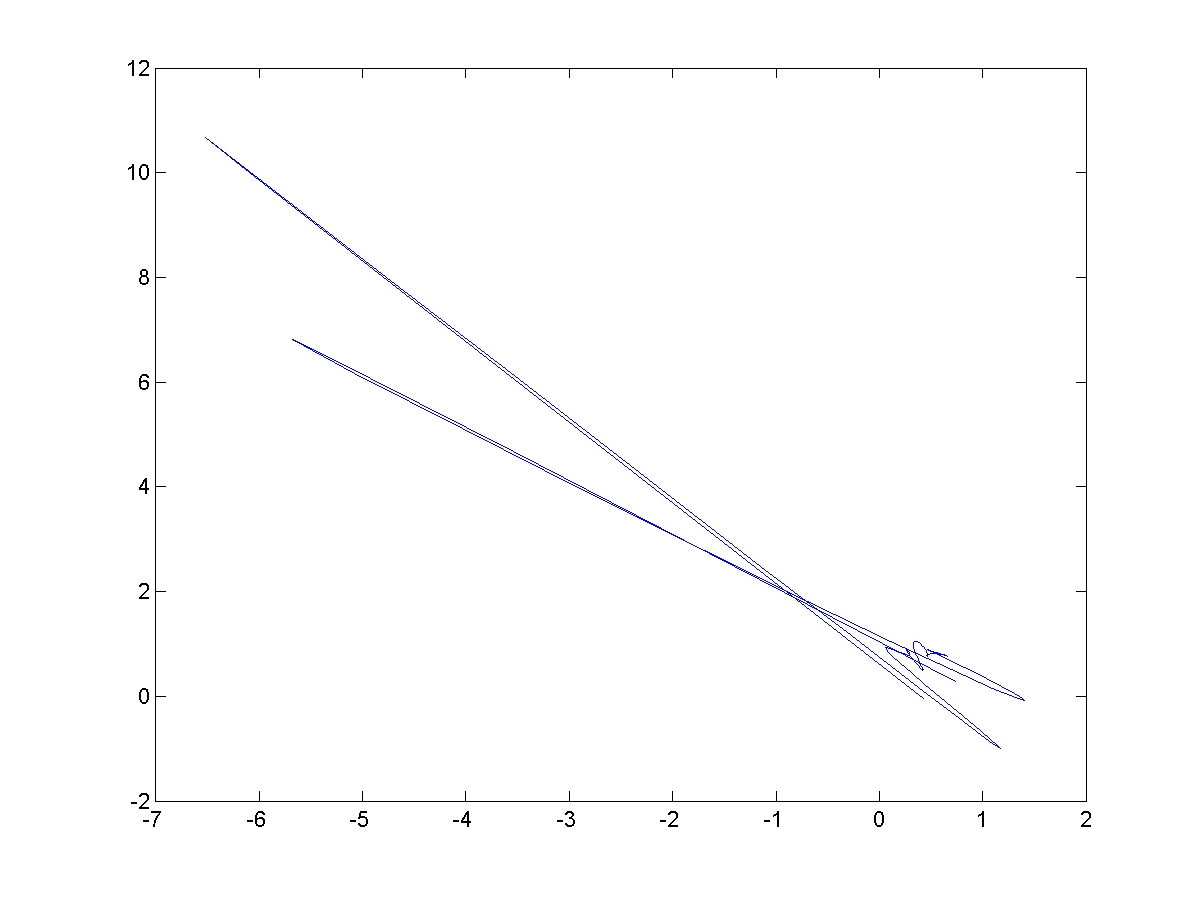
\includegraphics[width=\textwidth]{manointerpolada.jpg}
\begin{center}
Observe las grandes oscilaciones de los polinomios interpolantes en los extremos de la mano.
\end{center}
\end{enumerate}

\newpage
\item (20 pt.) Descargue el fichero ubicado en
\url{http://www.udec.cl/~fmilanese/MOP.csv}
este contiene los datos de inversi\'on realizadas por el MOP en distintas regiones de Chile desde el año 1991 hasta el 2014. 

En un mismo gr\'afico, grafique la inversi\'on anual realizada en la regiones Metropolitana y del Biob\'io, adem\'as grafique el polinomio interpolante de grado 1, 2 y 3 a cada conjunto de datos. Grabe la gr\'afica como \texttt{MOP.jpg} y adj\'untela al correo.

\textquestiondown Cuanto dinero a invertido el MOP desde 1995 en la regi\'on del Biobio?.

\textbf{Desarrollo:} El fichero \texttt{MOP.csv} contiene un encabezado con letras, removiendo este encabezado se puede leer usando \texttt{dlmread()}. El c\'odigo que genera la gr\'afica solicitada es

\begin{lstlisting}
clear all; clc; close all;
%% Leemos los datos
DATA=dlmread('MOP_sinencabezado.csv');
ANHOS=DATA(:,1);
BIOBIO=DATA(:,11);
METROPOLITANA=DATA(:,8);
%%Graficamos lo pedido
plot(ANHOS,BIOBIO,ANHOS,METROPOLITANA);
hold all;
%% Calculamos los interpolantes pedidos
    P1BIOBIO=polyfit(ANHOS,BIOBIO,1);
    P2BIOBIO=polyfit(ANHOS,BIOBIO,2);
    P3BIOBIO=polyfit(ANHOS,BIOBIO,3);
    P1METROPOLITANA=polyfit(ANHOS,METROPOLITANA,1);
    P2METROPOLITANA=polyfit(ANHOS,METROPOLITANA,2);
    P3METROPOLITANA=polyfit(ANHOS,METROPOLITANA,3);
 %% Graficamos los interpolantes
 pause
    vectorDIBUJO=1991:0.3:2014;
    plot(   vectorDIBUJO,polyval(P1BIOBIO,vectorDIBUJO),...
            vectorDIBUJO,polyval(P2BIOBIO,vectorDIBUJO),...
            vectorDIBUJO,polyval(P3BIOBIO,vectorDIBUJO),...
            vectorDIBUJO,polyval(P1METROPOLITANA,vectorDIBUJO),...
            vectorDIBUJO,polyval(P2METROPOLITANA,vectorDIBUJO),...
            vectorDIBUJO,polyval(P3METROPOLITANA,vectorDIBUJO) );

legend( 'Inversion Biobio',...
        'Inversion Metropolitana',...
        'P1 Biobio',...
        'P2 Biobio',...
        'P3 Biobio',...
        'P1 Metropolitana',...
        'P2 Metropolitana',...
        'P3 Metropolitana'  );
        
%Grabamos la grafica
print('-djpeg99','MOP');

%% Inversion desde 1995 en la region.
total=sum(BIOBIO(5:end,:));
money=cur2str(total)
\end{lstlisting}

y la gr\'afica \texttt{MOP.jpg} generada es

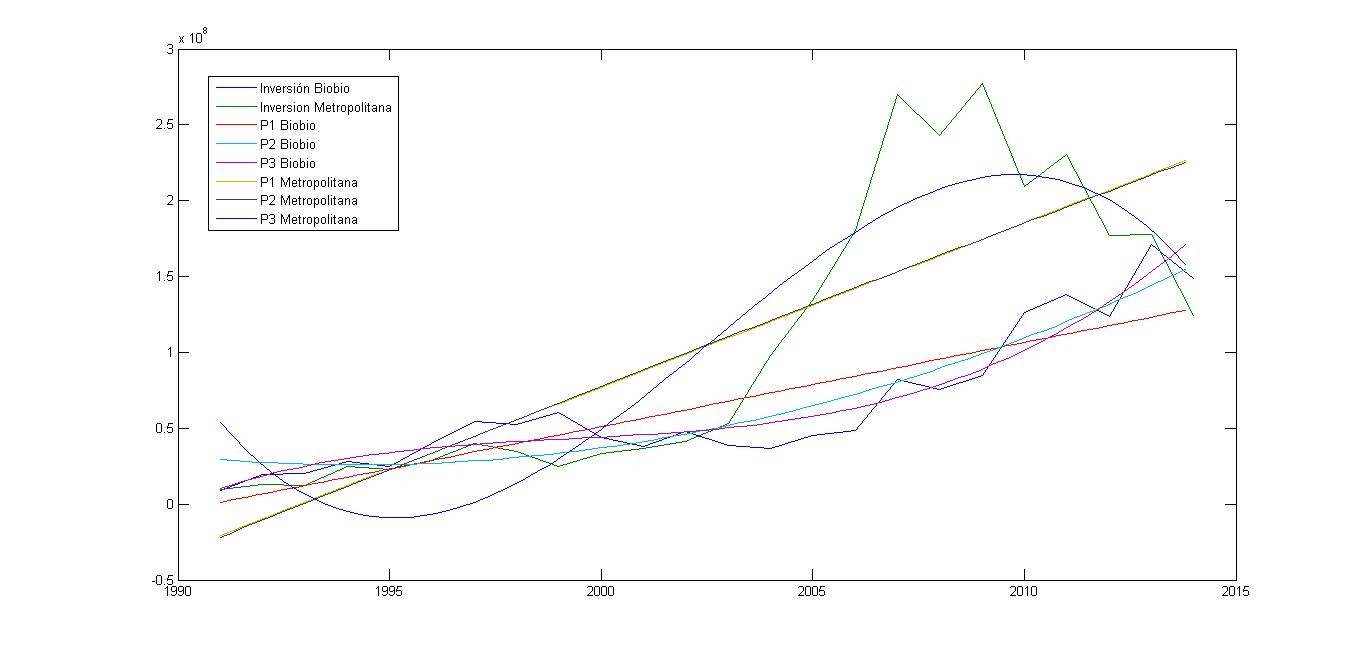
\includegraphics[width=\textwidth]{MOP2.jpg}


\end{enumerate}
\end{document}   